\documentclass[12pt]{article}

\usepackage[a4paper, margin=1in]{geometry}
\usepackage{xcolor}
\usepackage{tcolorbox}
\usepackage{fontawesome5} % icons
\usepackage{hyperref}
\usepackage{graphicx}
\usepackage{comment}
\usepackage[nameinlink,capitalize,noabbrev]{cleveref}
\usepackage{subcaption} % modern replacement for the deprecated subfigure package

\setlength{\parindent}{0pt}

% --- COLOR PALETTE (customize these) ---
\definecolor{maincolor}{HTML}{2A9D8F} % your teal
\definecolor{accentcolor}{HTML}{E76F51}
\definecolor{lightcolor}{HTML}{FFDEAD}

% Tell cleveref how to name your counter
\crefname{exercise}{assignment}{assignments}
\Crefname{exercise}{Assignment}{Assignments}

% --- ASSIGNMENT STYLE ---
\newcounter{exercise}

% Optional label: \exercisetitle[<label>]{<Title>}
\newcommand{\exercisetitle}[2][]{%
  \refstepcounter{exercise}% make this step referenceable/hyperlinked
  \vspace{0.5cm}%
  \colorbox{maincolor}{%
    \makebox[\dimexpr\linewidth-2\fboxsep][l]{%
      \textcolor{white}{\faPen\ Assignment \theexercise:~ #2}%
    }%
  }%
  % If an optional label was provided, set it
  \if\relax\detokenize{#1}\relax\else\label{#1}\fi
  \vspace{0.3cm}%
}


% --- IMPORTANT BOX ---
\newtcolorbox{importantbox}{
  colback=lightcolor,
  colframe=accentcolor,
  arc=4mm,
  boxrule=1pt,
  left=6pt,
  right=6pt,
  top=6pt,
  bottom=6pt
}

% --- PROMPT BOX ---
\newtcolorbox{promptbox}{
  colback=white,
  colframe=maincolor,
  arc=4mm,
  boxrule=1pt,
  left=6pt,
  right=6pt,
  top=6pt,
  bottom=6pt
}

% --- QUESTION BOX ---
\newcounter{question}

\newcommand{\question}[2][5cm]{%
  \stepcounter{question}
  \vspace{0.3cm}
  \textbf{\faEdit\ Question \thequestion: #2} \\[0.3em]
  
  \begin{Form}
  \TextField[
    name=Q\thequestion,
    multiline=true,
    width=\linewidth,
    height=#1,
    charsize=10pt,
    bordercolor={0 0 0},
    borderwidth=1.8,
    backgroundcolor={1 1 1}
  ]{}
  \end{Form}
  
  \vspace{0.3cm}
}

% --- SOLUTION BOX ---
%--- Definition of solution/no solution env to change between the teacher and the student versions --------%

% --- Teacher toggle ---
\newif\ifteacher
\teachertrue  % Write teacherfalse for student version and teachertrue for teachers version

% --- Solution environment ---
\newtcolorbox{solutionbox}{colback=gray!10,colframe=black!60!black,arc=1mm,boxrule=1pt}

\ifteacher
\newenvironment{solution}{%
  \begin{solutionbox}\textbf{Solution:}
}{%
  \end{solutionbox}
}
\else
  \excludecomment{solution}
\fi


\begin{document}

\begin{titlepage}

% --- Top spacing ---
\vspace*{2cm}

% --- Title page ---
\begin{center}
    {\Huge \bfseries \color{maincolor} From noise to narrative \par}
    \vspace{0.5cm}
    
    {\Large \color{accentcolor} Teaching with AI (TAI) \par}
    
    \vspace{1.5cm}
    
    \begin{center}
{\large
Mirte van der Eyden$^{1}$, Andrea López Incera$^{2}$ \\[0.3cm]

{\small
$^{1}$ Institut für Fachdidaktik, Universität Innsbruck \\ 
mirte.van-der-eyden@uibk.ac.at \\[0.2cm]


$^{2}$ Departament de didàctica de la matemàtica i les ciències experimentals, Universitat Autònoma de Barcelona \\ 
andrea.lopez.incera@uab.cat
}
}
\end{center}

\end{center}

\vfill

% --- Logos at the bottom ---
\begin{center}
\begin{tabular}{ccc}

\includegraphics[height=1.5cm]{Figures/Logos/universitaet-innsbruck-logo-cmyk-farbe.jpg} &

\includegraphics[height=1.5cm]{Figures/Logos/logotipuab-v1-verd.png} &

\includegraphics[height=1.5cm]{Figures/Logos/EN Co-funded by the EU_POS.jpg}
\end{tabular}
\end{center}


\vspace{0.5cm}

% Optional footer text
\begin{center}
    {\small Project funded by Erasmus+ Programme of the European Union}
\end{center}

\end{titlepage}

% --- Description of activity ---
\vspace*{0.5\textheight}

Subject: Sound generation with AI

Activity duration: 90 min

\vspace{0.5cm}

Steps:
\begin{enumerate}
    \item Initial discussion and explanation: from noise to sound (10 min)
    \item Recreating a classroom sound (10 min)
    \item Assignment 1: sound effects under video (60 min)
    \item Share results and reflect (10 min)
\end{enumerate}

Learning goals:

\begin{itemize}
    \item How diffusion models can be used to generate sound. 
    \item How to write prompts to generate sound. 
    \item The importance of sound effects and ambient sound for a video. 
\end{itemize}

Setup: 
\begin{itemize}
    \item Per 1-3 students a computer with internet access and headphones. 
    \item Accounts for an AI sound generation tool, e.g. Adobe Firefly. Free versions are available, but often have a limited number of generations.  
    \item One 30 second video without sound for every group. 
\end{itemize}

\newpage

% --- HEADER / BRANDING ---
\begin{center}
    {\Huge \color{maincolor} From noise to narrative}\\[5pt]
    {\large \textit{Generating sound effects with AI}}\\
    \rule{\linewidth}{1pt}
\end{center}

\vspace{0.5cm}

In a video, the sound effects are as important as the images. In this lesson, you generate the sound behind a video using available AI tools.

\exercisetitle[]{Initial discussion}

Discuss the following questions in small groups or in class: 

\begin{itemize}
    \item What are your experiences with creating music or sound with AI?
    \item How do you think sound is generated by an AI?
\end{itemize}


\section{From noise to sound with diffusion}

In the lesson on diffusion models, you learned how these models are used to create images out of noise. Similar models can be used to create sound out of noise.

Sounds are defined by their audio waveform or spectrograms. For example, \cref{fig:audio_waveform} shows images of the audio waveform belonging to a snare and kick sound of a drum.


\begin{figure}[htbp]
  \centering
  \begin{subfigure}[t]{0.48\textwidth}
    \centering
    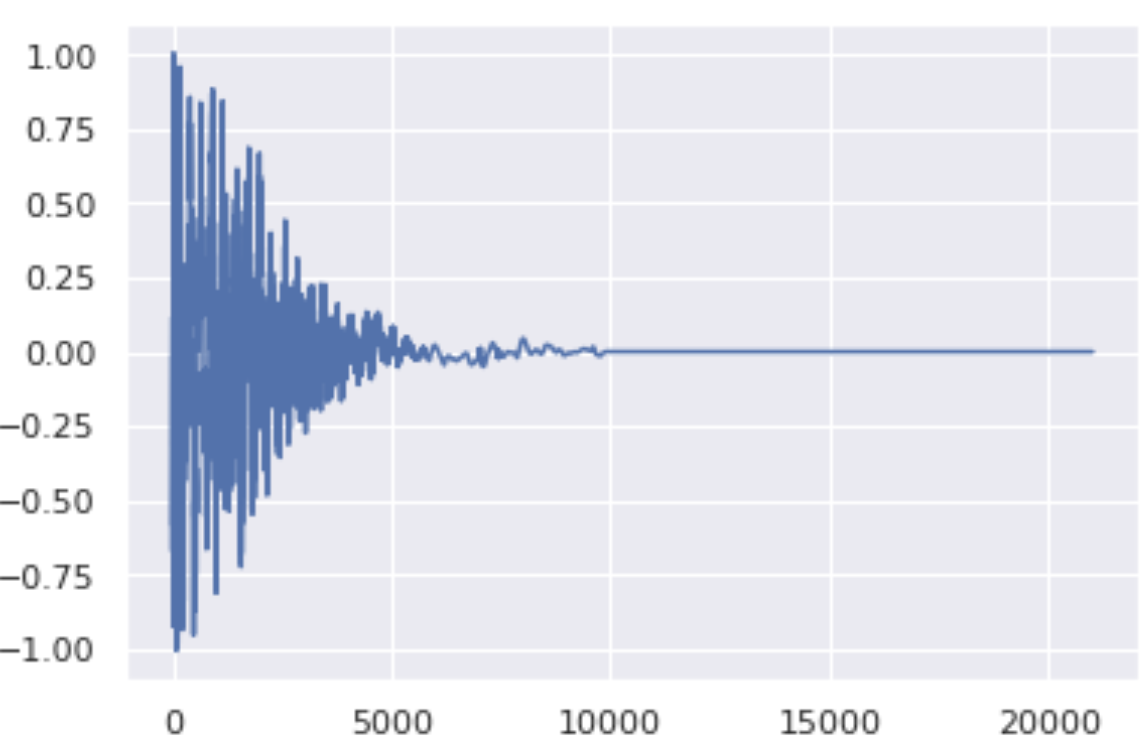
\includegraphics[width=\linewidth]{Figures/sound/snare_image.png}
    \caption{Snare drum.}
    \label{fig:snare}
  \end{subfigure}\hfill
  \begin{subfigure}[t]{0.48\textwidth}
    \centering
    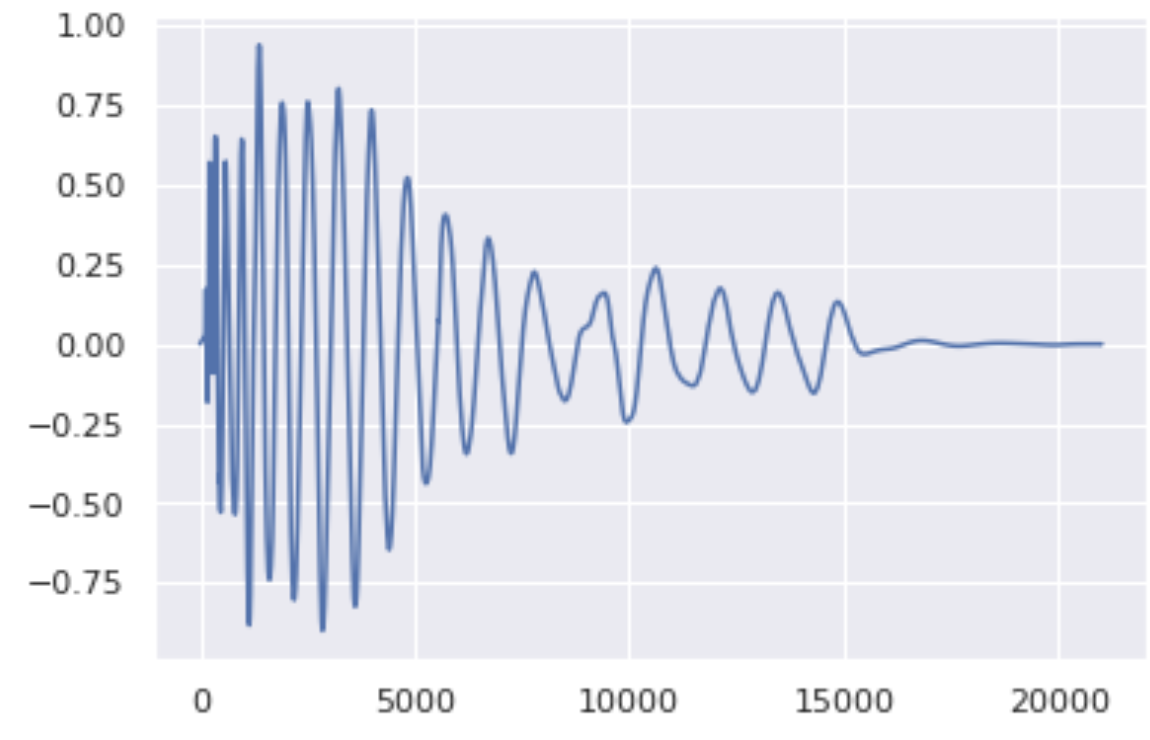
\includegraphics[width=\linewidth]{Figures/sound/kick_image.png}
    \caption{Kick drum.}
    \label{fig:kick}
  \end{subfigure}
  \caption{Examples of audio waveforms of sound. The y-axis shows the amplitude, the x-axis shows the time. Source: Rouard, Hadjeres 2021 \url{https://crash-diffusion.github.io/crash/}}
  \label{fig:audio_waveform}
\end{figure}

In case of images, the model learned to 'denoise' a noisy image by first applying forward diffusion to many images. With this, it learned how to reverse it.

For sound, this goes similarly. By adding noise to many structured sound recordings like the ones above, the diffusion model learns how to reverse the diffusion and regain a snare or kick sound.

Here you can see how the sounds of the snare and kick drum are retrieved from noise: \url{https://github.com/simonrouard/CRASH/blob/master/README.md}.

\exercisetitle[]{Generating and improving a classroom sound}

Form groups of 2/3 students and make sure you have an AI platform available where you can generate sound effects, such as Adobe Firefly (\url{https://firefly.adobe.com/generate/sound-effects}). 

\vspace{0.3cm}
\textcolor{maincolor}{\textbf{\faPen\ a) Make a classroom sound}} Use some objects that are around you to create a sound or sequence of sounds of maximally 8 seconds. Make sure that the sound is reproducible, and that it is not too loud or disturbing for your classmates. 

\question{Describe the sound in words.}


\vspace{0.3cm}
\textcolor{maincolor}{\textbf{\faPen\ b) Mimic the classroom sound}} Write a prompt to recreate the same sound with AI. 

\question{Write your first prompt here.}

You can compare the sound to the real sound. Try to make it as good as possible. 

\question{What was the best working prompt so far?}

\vspace{0.3cm}
\textcolor{maincolor}{\textbf{\faPen\ c) Improve your prompt }} 

Read the checklist below on how to write a good prompt for sound creation. 
\subsection*{Checklist: How to write a good prompt for sound creation}
As with text and images, you should be as specific as you can when writing a prompt for a sound effect. It helps to incorporate the following elements:
\begin{itemize}
  \item \textbf{Subject:} What is making the sound?
  \item \textbf{Action:} What is the subject doing that creates the sound?
  \item \textbf{Material:} What substances or materials are interacting? Rain falling on the sea sounds different than on pavement. A wooden stick tapping on the concrete floor sounds different from a metal one tapping on a wooden floor.
  \item \textbf{Space:} Where is the situation happening? In a big empty space like a field, the echo/reverb is different than in a small room or a dense forest. Describe the space (small room, open field, large hall) to shape reverberation and distance.
  \item \textbf{Mood:} Descriptive words about the feeling the sound gives, e.g., “sudden”, “silent”, “aggressive”, “cautious”.
  \item \textbf{Duration:} How long does the sound last?
  \item \textbf{Build-up:} For example, “300 millisecond hit with fast decay”. If possible, it helps to input a voice recording where you mimic the build-up of the sound.
  \item \textbf{Loopability:} If you want the sound to loop seamlessly, add the term \emph{loopable} (e.g., continuous rain in the background).
\end{itemize}

\question[3cm]{Which aspects did you miss in your prompt? Do you think they can improve your sound?}

Use the checklist to write an improved prompt. 

\question{What was your final prompt?}



\exercisetitle{Sound effects with AI}

Make groups of 2–3 students. Each group chooses a 30 second video without sound. Create the sound effects behind it using an AI sound generation model (for example Adobe Firefly, or Canva). Afterwards, every group shows their result. 

Follow the workflow as described here in the assignment, and answer the questions. 

\vspace{0.3cm}
\textcolor{maincolor}{\textbf{\faPen\ a) Choose a video. }} 
Choose a video from the available files.

\question[2cm]{What title do you give to your video?}



\vspace{0.3cm}
\textcolor{maincolor}{\textbf{\faPen\ b) List the sounds.}} 

 Make a list of all the things in the video that make sound (e.g., the rain in the background, the cup on the table, the footsteps on the floor). Make a distinction between \emph{ambient} sound (music, continuous background sound) and \emph{sound effects} belonging to distinct events in the video.\\[0.3em]
\TextField[
  name=Q19,
  multiline=true,
  width=\linewidth,
  height=10cm,      % adjust height for long answers
  charsize=10pt,   % text size inside the box
  bordercolor={0 0 0},
  backgroundcolor={1 1 1}
]{}



\vspace{0.3cm}
\textcolor{maincolor}{\textbf{\faPen\ c) Create a timeline.}} 
Put all the sounds you want to make in a timeline. 

\TextField[
  name=Q20,
  multiline=true,
  width=\linewidth,
  height=5cm,      % adjust height for long answers
  charsize=10pt,   % text size inside the box
  bordercolor={0 0 0},
  backgroundcolor={1 1 1}
]{}


\vspace{0.3cm}
\textcolor{maincolor}{\textbf{\faPen\ d) Creating the sound. }}
Now, use an AI platform to create the sounds and put them behind the video. In Adobe Firefly, you can upload the video and add multiple audio tracks. 







\vspace{0.3cm}
\textcolor{maincolor}{\textbf{\faPen\ e) Present. }}
You will present the video in the class. Be prepared to answer the following questions in front of the group:
    \begin{itemize}
      \item With what sound effect are you happiest?
      \item Which sound effect was hard to make?
      \item Share one example of a prompt that you used. Which parts of that prompt did you add later and turned out to be important?
    \item Name one sound effect that has an influence on the mood of the video. 
    \end{itemize}



\vspace{0.3cm}
\textcolor{maincolor}{\textbf{\faPen\ e) Compare }} 
If available, your teacher can provide you with the version of the video with sound. Compare it to your creation. 

\question{What were the largest differences?}


\exercisetitle[]{Final discussion}


    \begin{itemize}
      \item What is the importance of sound for a video?
      \item Apart from sound effects in videos, do you see other applications of this tool?
      \item What are the pros and cons of creating sound effects with AI?
\end{itemize}




\end{document}